\documentclass[a4paper,11pt]{article}
\usepackage[utf8]{inputenc}
\usepackage[T1]{fontenc}
\usepackage[swedish]{babel}
\usepackage{amsmath,amssymb,amsfonts}
\usepackage{tikz}
\usepackage{pgfplots} % För snygga och flexibla grafer
\pgfplotsset{compat=1.17} % Anpassa version vid behov
\usepackage{enumitem}
\usepackage{geometry}
\geometry{margin=2.5cm}

\title{Prövning Matematik 1b}
\author{Partille Gymnasium}
\date{11 september 2025}

\begin{document}

\maketitle

\begin{center}
\fbox{\parbox{0.93\textwidth}{
\textbf{Information och regler:}\\
\vspace{2mm}
\begin{itemize}[leftmargin=*,nosep]
    \item Du \textbf{får använda} miniräknare, linjal och formelblad.
    \vspace{2mm}
    \item Mobiltelefoner och andra kommunikationsmedel är \textbf{inte tillåtna}.
    \vspace{2mm}
    \item Tystnad gäller i provsalen.
    \vspace{2mm}
    \item Svara tydligt och visa alla uträkningar på ett \textbf{separat papper}.
    \vspace{2mm}
    \item Provet består av \textbf{två delar}, men samma regler gäller för bägge delarna.
    \vspace{2mm}
    \item \textbf{Inga toabesök}, utom mellan delarna. Du får då inte tillbaka din första del.
    \vspace{2mm}
    \item Misstänkt fusk kommer resultera i att provet inte kan bedömmas.
\end{itemize}
\vspace{2mm}
}}
\end{center}

\begin{center}
\fbox{\parbox{0.93\textwidth}{
Jag skriver under på att jag tagit del av reglerna ovan och följer dem:

\vspace{2mm}
\textbf{Namn:}\hrulefill\hspace{1cm}\textbf{Klass:}\hrulefill
}}
\end{center}

\newpage
\section*{Del B}
\begin{enumerate}
    \item Lös ekvationen: $\frac{3y}{2} -2 = y + 4$
    \item Faktorisera uttrycket: $6x^2y + 9xy^2$
    \item En rät linje går genom punkterna (2,3) och (5,9). Bestäm linjens ekvation på formen $y = kx + m$.
    \item I en låda finns 5 röda och 3 blå kulor. Du tar två kulor ur lådan utan att lägga tillbaka den första.
    \begin{enumerate}[label=\alph*)]
      \item Vad är sannolikheten att du tar två röda kulor?
      \item Vad är sannolikheten att du tar en röd och en blå kula?
    \end{enumerate}
    \item Nedan visas grafen till en linjär funktion.
    \begin{enumerate}[label=\alph*)]
        \item Vad är lutningen för linjen?
        \item Bestäm linjens ekvation på formen $y = kx + m$.
    \end{enumerate}
    \begin{center}
    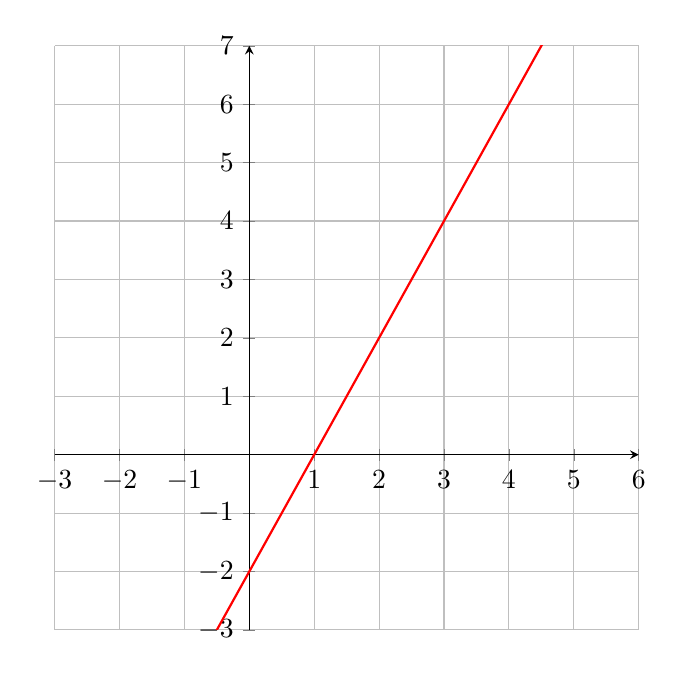
\begin{tikzpicture}
      \begin{axis}[
        axis lines=middle,
        axis line style/.append style={-},
        grid=both,
        xmin=-3, xmax=6,
        ymin=-3, ymax=7,
        samples=200,
        width=9cm,
        height=9cm,
        domain=-2:5,
        xtick distance=1,
        ytick distance=1,
        clip=true
      ]
        \addplot[red, thick] {2*x - 2 };
      \end{axis}
    \end{tikzpicture}
    \end{center}
    \item Viktor har köpt en begagnad mobiltelefon. Priset på telefonen kan beräknas med formeln $y=8000 \cdot 0.8^x$ där $x$ är antalet år sedan telefonen var ny.
    \begin{enumerate}[label=\alph*)]
      \item Vad kostade telefonen när den var ny?
      \item När Viktor köpte den var telefonen 3 år gammal, hur mycket betalade han för den?
      \item Hur mycket minskar priset på telefonen per år i procent?
    \end{enumerate}
    \item En taxi kostar 45 kr i startavgift och därefter 15 kr per kilometer. 
    \begin{enumerate}[label=\alph*)]
      \item Skriv en formel för totalkostnaden $K(x)$ om du åker $x$ kilometer.
      \item Använd formeln för att beräkna kostnaden för en resa som är 5 kilometer lång.
      \item Använd formeln för att beräkna hur långt du kan resa för 165 kr.
    \end{enumerate}
    \end{enumerate}
\end{document}
